\documentclass[twocolumn]{article}
\usepackage[utf8]{inputenc}
\usepackage[english]{babel}
\usepackage{lipsum}
\usepackage{multicol}
\usepackage{abstract} % Allows abstract customization
\usepackage{footnote}
\usepackage{listings}
\usepackage{url}
\usepackage{dblfnote}
\usepackage{graphicx}
\usepackage[margin=1in]{geometry}
\usepackage{cite}
\usepackage{natbib}
\usepackage{amsmath}
\usepackage{algorithm}
\usepackage[noend]{algpseudocode}
\usepackage[]{units}

\graphicspath{ {../images/} }
\bibliographystyle{acm} 
\setlength{\columnsep}{1cm}

\begin{document}

\twocolumn[\begin{@twocolumnfalse}
  \centerline{\Large\bfseries Breaking Petya - Solving Malware Using a Poor Implementation of Salsa20}
  \vspace{3ex}
  \centerline{Peixian Wang}
  \centerline{May 6, 2016}
  \vspace{3ex}
  
  \begin{abstract}
	  Ransomware has become a relatively profitable development in recent years with the surge in popularity of Bitcoin and other untracable forms of money transactions. In this paper we detail Petya, a recent form of ransomware targeting Windows platforms and NTFS drives. We describe the construction of Petya and the underlying encryption algorithm, Salsa20, and also present one possible solution utilizing Z3, an efficient satisfiabliity modulo theory solver, to defeat Petya. 
  \end{abstract}
   \vspace{3ex}
\end{@twocolumnfalse}]

\section{Introduction}
Online transactions through Tor \cite{tor} using anonomyous cryptocurrencies allow for a certain level of privacy when it comes to payments, but also allow themselves to be used in a malicious fashion. Since Bitcoin, the most popular form of cryptocurrency, makes it extremely hard to track the transactions, Bitcoin has become the de facto standard for ransomware, malware which infects the victim's computer, holds files hostage through encryption, and extorts the victims for money in return for the files. Petya is one such ransomware, except rather than targeting the files of the victim, it targets the master boot record (MBR) and master file table (MFT) \cite{decryptPetya}.

\section{Petya}
\subsection{Overview}
Petya is a relatively new ransomware variant, only starting to appear within the early months of 2016. In order to bypass the lengthy process of encrypting each file on the victim's hard drive, Petya simply seeks to write malicious code to the start of the disk. This code overwrites the MBR of the hard drive with a small kernel that then encrypts the MFT. 
\subsection{Behavioral Analysis}
\begin{figure}
	
\includegraphics{petya.png}
	\caption{The petya executable disguised as a .pdf file.}
	\label{fig:petya}
\end{figure}
\begin{figure}
	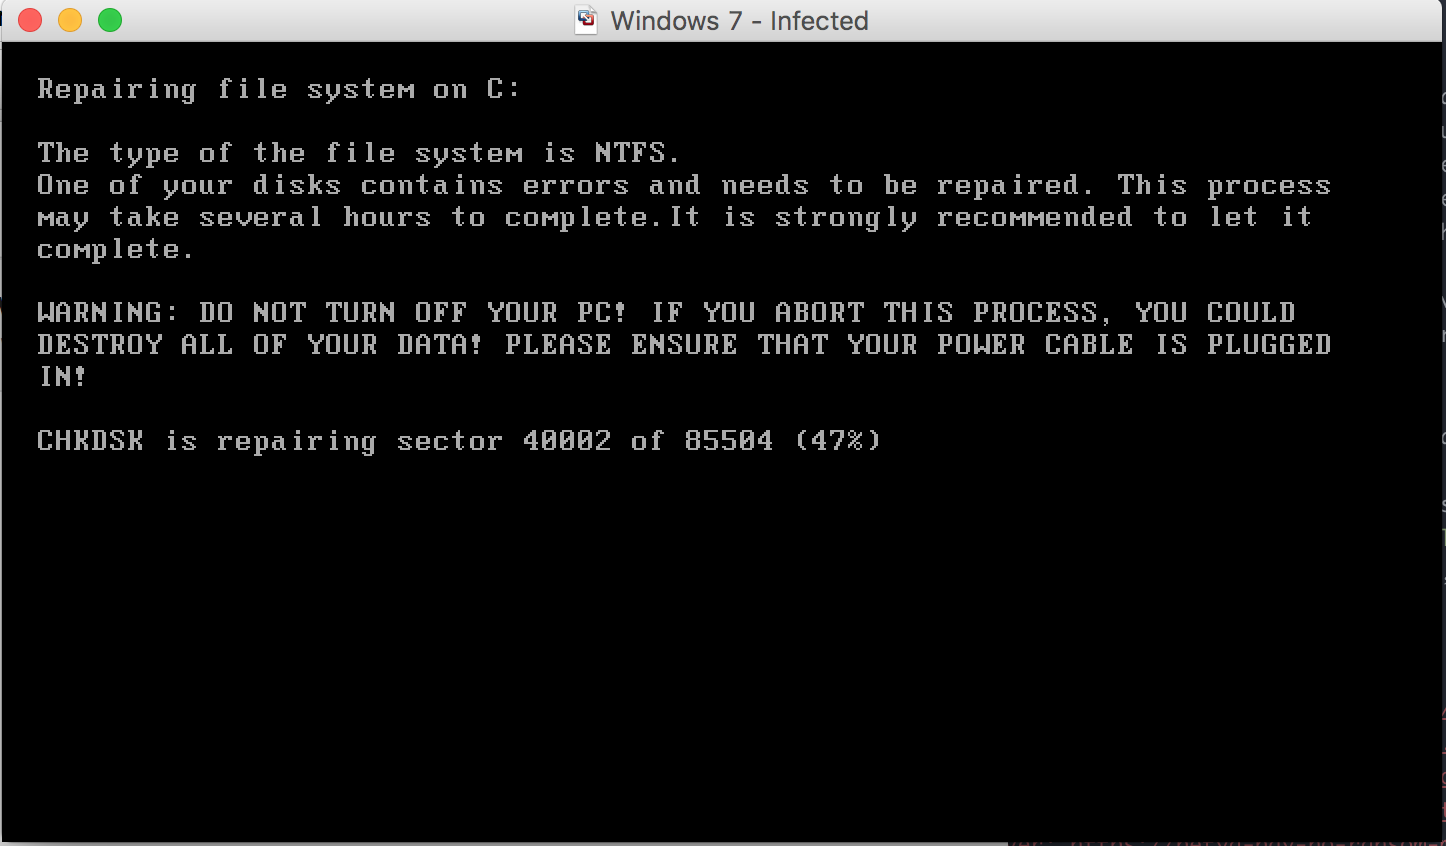
\includegraphics[width = 0.5\textwidth]{encryptionScreen.png}
	\caption{The fake CHKDSK scan made by Petya while it encrypts the MFT.}
	\label{fig:fakechk}
\end{figure}
\begin{figure}
	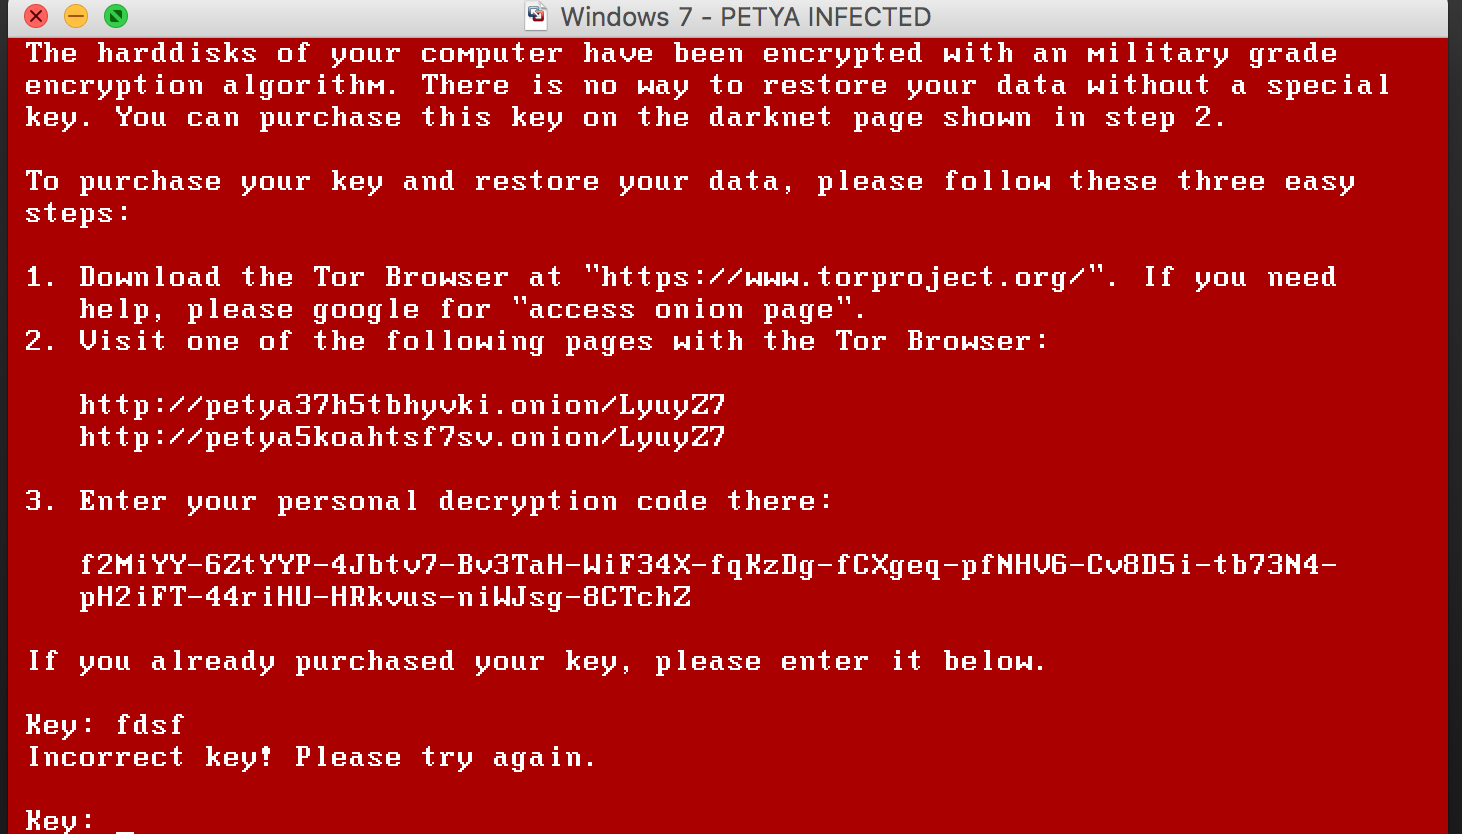
\includegraphics[width = 0.5\textwidth]{ransomScreen.png}
	\caption{The ransom note by Petya.}
	\label{fig:ransomScreen}
\end{figure}
\begin{figure}
	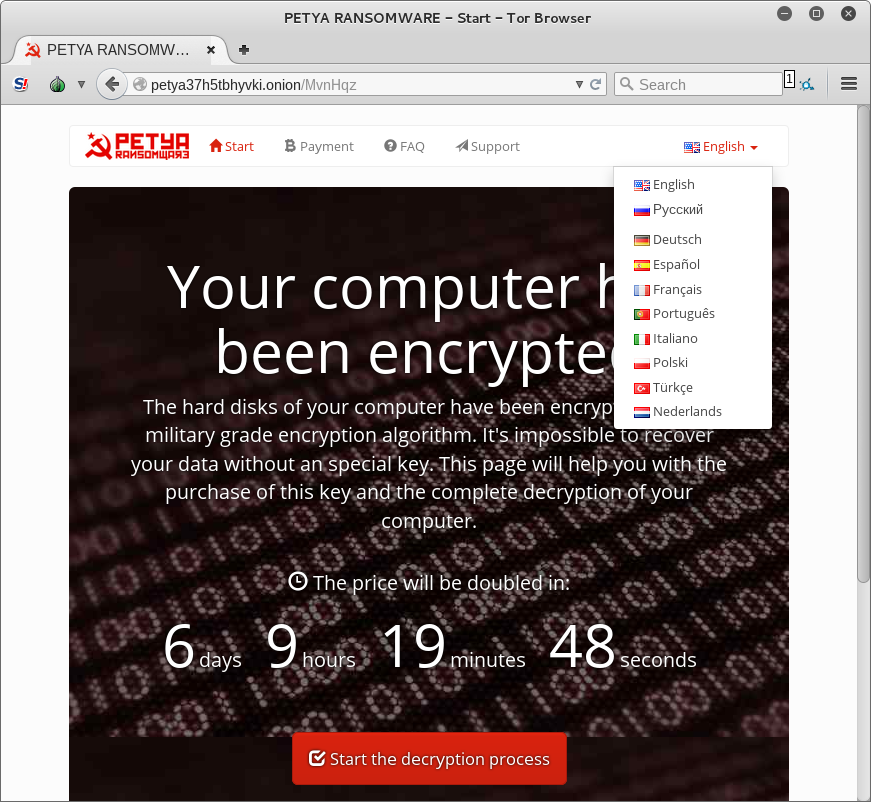
\includegraphics[width = 0.5\textwidth]{victimSite.png}
	\caption{Accessibility is important, even for malware. From \cite{lowLevelPetya}.}
	\label{fig:victimSite}
\end{figure}
\begin{figure}
	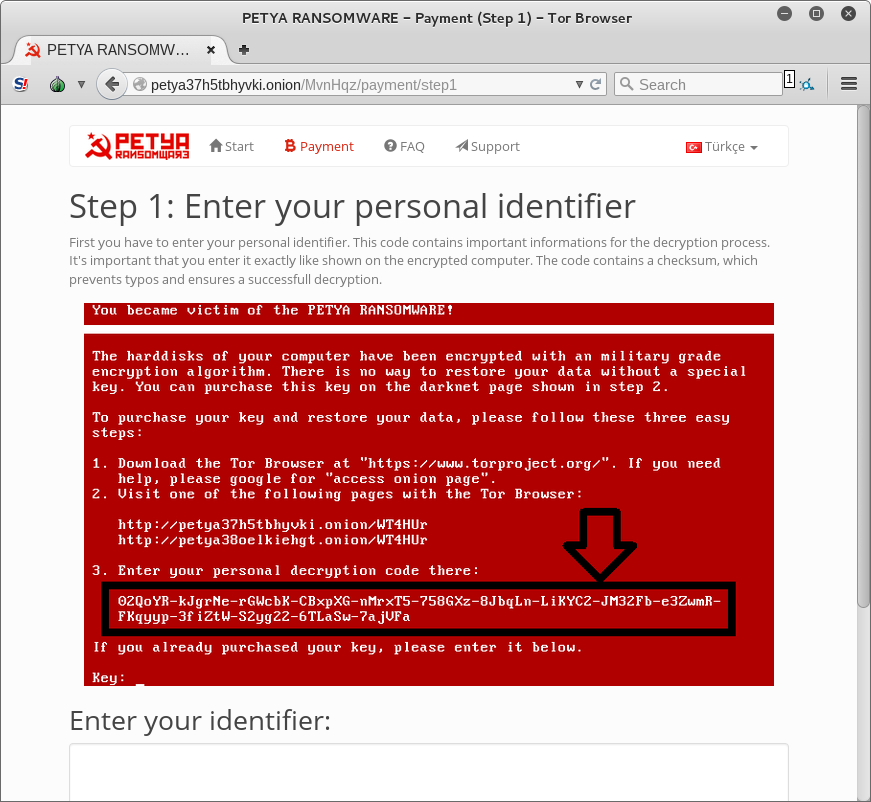
\includegraphics[width = 0.5\textwidth]{victimTutorial.png}
	\caption{Petya Tutorial on purchasing bitcoins and performing a transaction. }
	\label{fig:victimTutorial}
\end{figure}
Petya is usually destributed through a zip file \cite{lowLevelPetya}, containing two other files: 1. a photo of a young man, puporting to be an applicant and 2. an executable, disguised as a csv file, shown in figure \ref{fig:petya}. 
After opening the executable, Petya calls an undocumented API called NtRaiseHardError. The computer then promptly crashes and boots into a fake CHKDSK scan, shown in figure \ref{fig:fakechk}, which starts the encryption on the MFT. When the encryption completes, the user is shown a ransom note screen, shown in figure \ref{fig:ransomScreen}. After visiting the website, the user is presented with a relatively upscale website, featuring multiple languages (figure \ref{fig:victimSite}) and a tutorial on how victims can perform a bitcoin transaction (figure \ref{fig:victimTutorial}). 
\subsection{Code Analysis}

\section{Salsa20}
\subsection{Overview}
\subsection{Implementation}
\subsection{Implementation Within Petya}

\section{Infestor}
\subsection{Code Walkthrough}


As online transcations through Tor \cite{tor} and cryptocurrencies become more commonplace, 
\bibliography{paper} 

\end{document}